% Soubory musí být v kódování, které je nastaveno v příkazu \usepackage[...]{inputenc}

\documentclass[%        Základní nastavení
  %draft,    				  % Testovací překlad
  12pt,       				% Velikost základního písma je 12 bodů
	t,                  % obsah slajdů bude vždy začínat od shora (nebude vertikálně centrovaný)
	aspectratio=1610,   % poměr stran bude 16:10 (všechny projektory v učebnách na Technické 12 Brno),
	                    % další volby jsou 43, 149, 169, 54, 32.
	unicode,						% Záložky a informace budou v kódování unicode
]{beamer}				    	% Dokument třídy 'zpráva', vhodná pro sazbu závěrečných prací s kapitolami
%\usepackage{etex}

\usepackage[utf8]		  % Kódování zdrojových souborů je v UTF-8
	{inputenc}					% Balíček pro nastavení kódování zdrojových souborů
	
\usepackage{graphicx} % Balíček 'graphicx' pro vkládání obrázků
											% Nutné pro vložení logotypů školy a fakulty

\usepackage[          % Balíček 'acronym' pro sazby zkratek a symbolů
	nohyperlinks				% Nebudou tvořeny hypertextové odkazy do seznamu zkratek
]{acronym}						
											% Nutné pro použití prostředí 'acronym' balíčku 'thesis'

%% Balíček hyperref je volán třídou beamer automaticky, proto není třeba následujícího kódu:
%\usepackage[
%	breaklinks=true,		% Hypertextové odkazy mohou obsahovat zalomení řádku
%	hypertexnames=false % Názvy hypertextových odkazů budou tvořeny
%											% nezávisle na názvech TeXu
%]{hyperref}						% Balíček 'hyperref' pro sazbu hypertextových odkazů
%											% Nutné pro použití příkazu 'nastavenipdf' balíčku 'thesis'

\usepackage{cmap} 		% Balíček cmap zajišťuje, že PDF vytvořené `pdflatexem' je
											% plně "prohledávatelné" a "kopírovatelné"

%\usepackage{upgreek}	% Balíček pro sazbu stojatých řeckých písmem
											%% např. stojaté pí: \uppi
											%% např. stojaté mí: \upmu (použitelné třeba v mikrometrech)
											%% pozor, grafická nekompatibilita s fonty typu Computer Modern!

%\usepackage{amsmath} %balíček pro sabu náročnější matematiky

\usepackage{booktabs} % Balíček, který umožňuje v tabulce používat
                      % příkazy \toprule, \midrule, \bottomrule


%%%%%%%%%%%%%%%%%%%%%%%%%%%%%%%%%%%%%%%%%%%%%%%%%%%%%%%%%%%%%%%%%
%%%%%%      Definice informací o dokumentu             %%%%%%%%%%
%%%%%%%%%%%%%%%%%%%%%%%%%%%%%%%%%%%%%%%%%%%%%%%%%%%%%%%%%%%%%%%%%

% V tomto souboru se nastavují téměř veškeré informace, proměnné mezi studenty:
% jméno, název práce, pohlaví atd.
% Tento soubor je SDÍLENÝ mezi textem práce a prezentací k obhajobě -- netřeba něco nastavovat na dvou místech.
\usepackage{url}
\usepackage{makecell}
\usepackage[
%%% Z následujících voleb jazyka lze použít pouze jednu
  %czech-english,		% originální jazyk je čeština, překlad je anglicky (výchozí)
  %english-czech,	% originální jazyk je angličtina, překlad je česky
  %slovak-english,	% originální jazyk je slovenština, překlad je anglicky
  english-slovak,	% originální jazyk je angličtina, překlad je slovensky
%
%%% Z následujících voleb typu práce lze použít pouze jednu
  semestral,		  % semestrální práce (nesází se abstrakty, prohlášení, poděkování) (výchozí)
  %bachelor,			%	bakalářská práce
  %master,			  % diplomová práce
  %treatise,			% pojednání o disertační práci
  %doctoral,			% disertační práce
%
%%% Z následujících voleb zarovnání objektů lze použít pouze jednu
%  left,				  % rovnice a popisky plovoucích objektů budou zarovnány vlevo
	center,			    % rovnice a popisky plovoucích objektů budou zarovnány na střed (vychozi)
%
]{thesis}   % Balíček pro sazbu studentských prací

%%% Jméno a příjmení autora ve tvaru
%  [tituly před jménem]{Křestní}{Příjmení}[tituly za jménem]
% Pokud osoba nemá titul před/za jménem, smažte celý řetězec '[...]'
\author[Bc.]{Jakub}{Senčák}

%%% Identifikační číslo autora (VUT ID)
\butid{196504}

%%% Pohlaví autora/autorky
% (nepoužije se ve variantě english-czech ani english-slovak)
% Číselná hodnota: 1...žena, 0...muž
\gender{0}

%%% Jméno a příjmení vedoucího/školitele včetně titulů
%  [tituly před jménem]{Křestní}{Příjmení}[tituly za jménem]
% Pokud osoba nemá titul před/za jménem, smažte celý řetězec '[...]'
\advisor[Ing.]{Adrián}{Tomášov}

%%% Jméno a příjmení oponenta včetně titulů
%  [tituly před jménem]{Křestní}{Příjmení}[tituly za jménem]
% Pokud osoba nemá titul před/za jménem, smažte celý řetězec '[...]'
% Nastavení oponenta se uplatní pouze v prezentaci k obhajobě;
% v případě, že nechcete, aby se na titulním snímku prezentace zobrazoval oponent, pouze příkaz zakomentujte;
% u obhajoby semestrální práce se oponent nezobrazuje (jelikož neexistuje)
% U dizertační práce jsou typicky dva až tři oponenti. Pokud je chcete mít na titulním slajdu, prosím ručně odkomentujte a upravte jejich jména v definici "VUT title page" v souboru thesis.sty.
\opponent[doc.\ Ing.]{Jan}{Hajný}[Ph.D.]

%%% Název práce
%  Parametr ve složených závorkách {} je název v originálním jazyce,
%  parametr v hranatých závorkách [] je překlad (podle toho jaký je originální jazyk).
%  V případě, že název Vaší práce je dlouhý a nevleze se celý do zápatí prezentace, použijte příkaz
%  \def\insertshorttitle{Zkác.\ náz.\ práce}
%  kde jako parametr vyplníte zkrácený název. Pokud nechcete zkracovat název, budete muset předefinovat,
%  jak se vytváří patička slidu. Viz odkaz: https://bit.ly/3EJTp5A
\title[Distributed acoustic sensing system data analysis applied for perimeter protection]{Distributed acoustic sensing system data analysis applied for perimeter protection}

%%% Označení oboru studia
%  Parametr ve složených závorkách {} je název oboru v originálním jazyce,
%  parametr v hranatých závorkách [] je překlad
\specialization[Teleinformatics]{Teleinformatika}

%%% Označení ústavu
%  Parametr ve složených závorkách {} je název ústavu v originálním jazyce,
%  parametr v hranatých závorkách [] je překlad
%\department[Department of Control and Instrumentation]{Ústav automatizace a měřicí techniky}
%\department[Department of Biomedical Engineering]{Ústav biomedicínského inženýrství}
%\department[Department of Electrical Power Engineering]{Ústav elektroenergetiky}
%\department[Department of Electrical and Electronic Technology]{Ústav elektrotechnologie}
%\department[Department of Physics]{Ústav fyziky}
%\department[Department of Foreign Languages]{Ústav jazyků}
%\department[Department of Mathematics]{Ústav matematiky}
%\department[Department of Microelectronics]{Ústav mikroelektroniky}
%\department[Department of Radio Electronics]{Ústav radioelektroniky}
%\department[Department of Theoretical and Experimental Electrical Engineering]{Ústav teoretické a experimentální elektrotechniky}
\department[Department of Telecommunications]{Ústav telekomunikací}
%\department[Department of Power Electrical and Electronic Engineering]{Ústav výkonové elektrotechniky a elektroniky}

%%% Označení fakulty
%  Parametr ve složených závorkách {} je název fakulty v originálním jazyce,
%  parametr v hranatých závorkách [] je překlad
%\faculty[Faculty of Architecture]{Fakulta architektury}
\faculty[Faculty of Electrical Engineering and~Communication]{Fakulta elektrotechniky a~komunikačních technologií}
%\faculty[Faculty of Chemistry]{Fakulta chemická}
%\faculty[Faculty of Information Technology]{Fakulta informačních technologií}
%\faculty[Faculty of Business and Management]{Fakulta podnikatelská}
%\faculty[Faculty of Civil Engineering]{Fakulta stavební}
%\faculty[Faculty of Mechanical Engineering]{Fakulta strojního inženýrství}
%\faculty[Faculty of Fine Arts]{Fakulta výtvarných umění}
%
%Nastavení logotypu (v hranatych zavorkach zkracene logo, ve slozenych plne):
\facultylogo[logo/FEKT\_zkratka\_barevne\_PANTONE\_CZ]{logo/UTKO_color_PANTONE_CZ}

%%% Rok odevzdání práce
\graduateyear{2023}
%%% Akademický rok odevzdání práce
\academicyear{2022/23}

%%% Datum obhajoby (uplatní se pouze v prezentaci k obhajobě)
\date{11.\,12.\,2022} 

%%% Místo obhajoby
% Na titulních stránkách bude automaticky vysázeno VELKÝMI písmeny (pokud tyto stránky sází šablona)
\city{Brno}

%%% Abstrakt
\abstract[%
Překlad abstraktu
(v~angličtině, pokud je originálním jazykem čeština či slovenština; v~češtině či slovenštině, pokud je originálním jazykem angličtina)
]{%
Abstrakt práce v~originálním jazyce
}

%%% Klíčová slova
\keywrds[%
Překlad klíčových slov
(v~angličtině, pokud je originálním jazykem čeština či slovenština; v~češtině či slovenštině, pokud je originálním jazykem angličtina)
]{%
Klíčová slova v~originálním jazyce
}

%%% Poděkování
\acknowledgement{%
I would like to thank my supervisor Ing.~Adrián Tomášov for leading me during my struggles with this work, for his time during our consultations and lots of patience. 
}%      % v tomto souboru doplňte údaje o sobě, o názvu práce...
                       % (tento soubor je sdílený s textem práce)

%%%%%%%%%%%%%%%%%%%%%%%%%%%%%%%%%%%%%%%%%%%%%%%%%%%%%%%%%%%%%%%%%%%%%%%%

%%%%%%%%%%%%%%%%%%%%%%%%%%%%%%%%%%%%%%%%%%%%%%%%%%%%%%%%%%%%%%%%%%%%%%%%
%%%%%%     Nastavení polí ve Vlastnostech dokumentu PDF      %%%%%%%%%%%
%%%%%%%%%%%%%%%%%%%%%%%%%%%%%%%%%%%%%%%%%%%%%%%%%%%%%%%%%%%%%%%%%%%%%%%%
%% Při vloženém balíčku 'hyperref' lze použít příkaz '\pdfsettings'
\pdfsettings
%  Nastavení polí je možné provést také ručně příkazem:
%\hypersetup{
%  pdftitle={Název studentské práce},    	% Pole 'Document Title'
%  pdfauthor={Autor studenstké práce},   	% Pole 'Author'
%  pdfsubject={Typ práce}, 						  	% Pole 'Subject'
%  pdfkeywords={Klíčová slova}           	% Pole 'Keywords'
%}
\hypersetup{pdfpagemode=FullScreen}       % otevření rovnou v režimu celé obrazovky
%%%%%%%%%%%%%%%%%%%%%%%%%%%%%%%%%%%%%%%%%%%%%%%%%%%%%%%%%%%%%%%%%%%%%%%

\usetheme{VUT} 				% barvy a rozložení prezentace odpovídající VUT FEKT
% alternativně lze použít jiná berevná témata, ale bez záruky. Například: 
%\usetheme{Darmstadt} \usecolortheme{default2}
\logoheader					% vytvoření zkráceného loga VUT FEKT v hlavičce slajdu, nechte odkomentované


\usepackage{dirtree}
\begin{document}

% v případě zakomentování následujícího se zobrazí v pravém dolním rohu slajdů klikatelné navigační symboly 
\disablenavigationsymbols

% titulní snímek, vysazen bez horních, dolních a postranních lišt (volba plain),
% není tak vysazen ani nadpis snímku
\maketitle

%%%%%%%%%%%%%%%%%%%%%%%%%%%%%%%%%%%%%%%%%%%%%%%%%%%%%%%%%%%%%%%%%%%%%%%
% 1. snímek s cíli (zadaním) práce
\begin{frame} 
	% nadpis snímku
	\frametitle{Ciele práce}
	\begin{itemize}
			\item Naštudovať problematiku systému DAS
			\item Popísať výstúpný formát - HDF5 
			\item Implementovať aplikáciu na prevod dát do WAV
			\item Spracovať možnosti aplikácie na analýzu dát v reálnom čase
	\end{itemize}
\end{frame}


% %%%%%%%%%%%%%
% \begin{frame} 
% 	\frametitle{Klíčové nástroje}

% 	% prostředí 'alertblock', které slouží pro zdůraznění informace
% 	\begin{alertblock}{Pro práci je klíčový Eulerův vzorec}
% 		$$\eul^{\jmag x}=\cos x + \jmag\sin x$$
% 	\end{alertblock}

% 	\vspace{4ex}
% 	Eulerova identita je speciálním případem tohoto vzorce, jestliže dosadíme $x=\uppi$\,:

% 	% prostředí 'block', které slouží jako informativní
% 	\begin{block}{Eulerova identita}
% 		$$\eul^{\jmag \uppi}=\cos \uppi + \jmag\sin \uppi,$$\\
% 		odkud vyplývá
% 		$$\eul^{\jmag \uppi}+1=0.$$
% 	\end{block}
% \end{frame} 




\begin{frame}
    \frametitle{Štruktúra súboru HDF5}
   
    {\small
    %
    \label{dir:filestructure}
    \dirtree{%.
    .1 /\DTcomment{root}.
    .2 Acquisition\DTcomment{Recorded data}.
    .3 Custom\DTcomment{Empty}.
    .3 Raw[0]\DTcomment{HDF5 group (3 members)}.
    .4 Custom\DTcomment{HDF5 group (1 members)}.
    .5 SampleCount\DTcomment{HDF5 dataset, shape (332032,), type "<i8">}.
    .4 RawData[0]\DTcomment{HDF5 dataset, shape (100, 332032), type "<i2">}.
    .4 RawDataTime\DTcomment{HDF5 dataset, shape (332032,), type "<i8">}.
    }
    }

    \begin{itemize}
        \item Binárny formát
        \item Abstraktný dátový model
        \item Vnútorný formát definovaný uživateľom
    \end{itemize}
\end{frame}

\begin{frame}{Frame Title}
    \frametitle{Prevod HDF5 do WAV}
    \begin{itemize}
        \item Python
        \item h5py, SciPy, numpy
        \item Analýza HDF5 a hľadanie datasetov
        \item Výber kanálu
        \item Interpolácia dát na správny rozsah podľa WAV formátu
        \item Prevzorkovanie - vzorkovacia frekvencia bola 10 kHz
        \item Pretypovanie na numpy.int16 - 16-bit PCM
    \end{itemize}
\end{frame}

\begin{frame}{Frame Title}
    \frametitle{Vizualizácia DAS dát}
    \begin{itemize}
        \item Existujúci software:
        \begin{itemize}
            \item OptaSense OS6
            \item h5web - ReactJS
        \end{itemize}
        \item Vlastnosti aplikácie:
        \begin{itemize}
            \item Multiplatformnosť
            \item Vizualizácia v reálnom čase
        \end{itemize}
        
        \item Nástroje:
        \begin{itemize}
            \item Python server
            \item Frontend = Svelte + D3js 
        \end{itemize}
    \end{itemize}
\end{frame}

\begin{frame}{Frame Title}
    \frametitle{Návrh aplikácie a jej súčasti}
    \begin{figure}
        \centering
        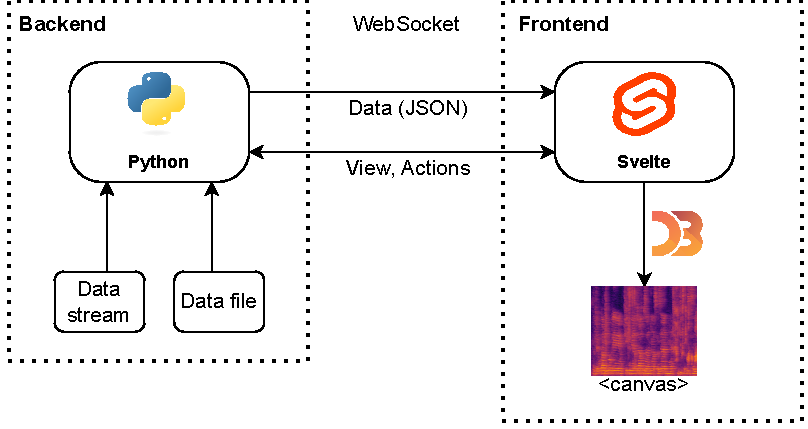
\includegraphics{obrazky/appstack.drawio.pdf}
        \label{fig:app_overview}
    \end{figure}
\end{frame}

\begin{frame}{Frame Title}
    \frametitle{Prototyp}
    \begin{figure}
        \centering
        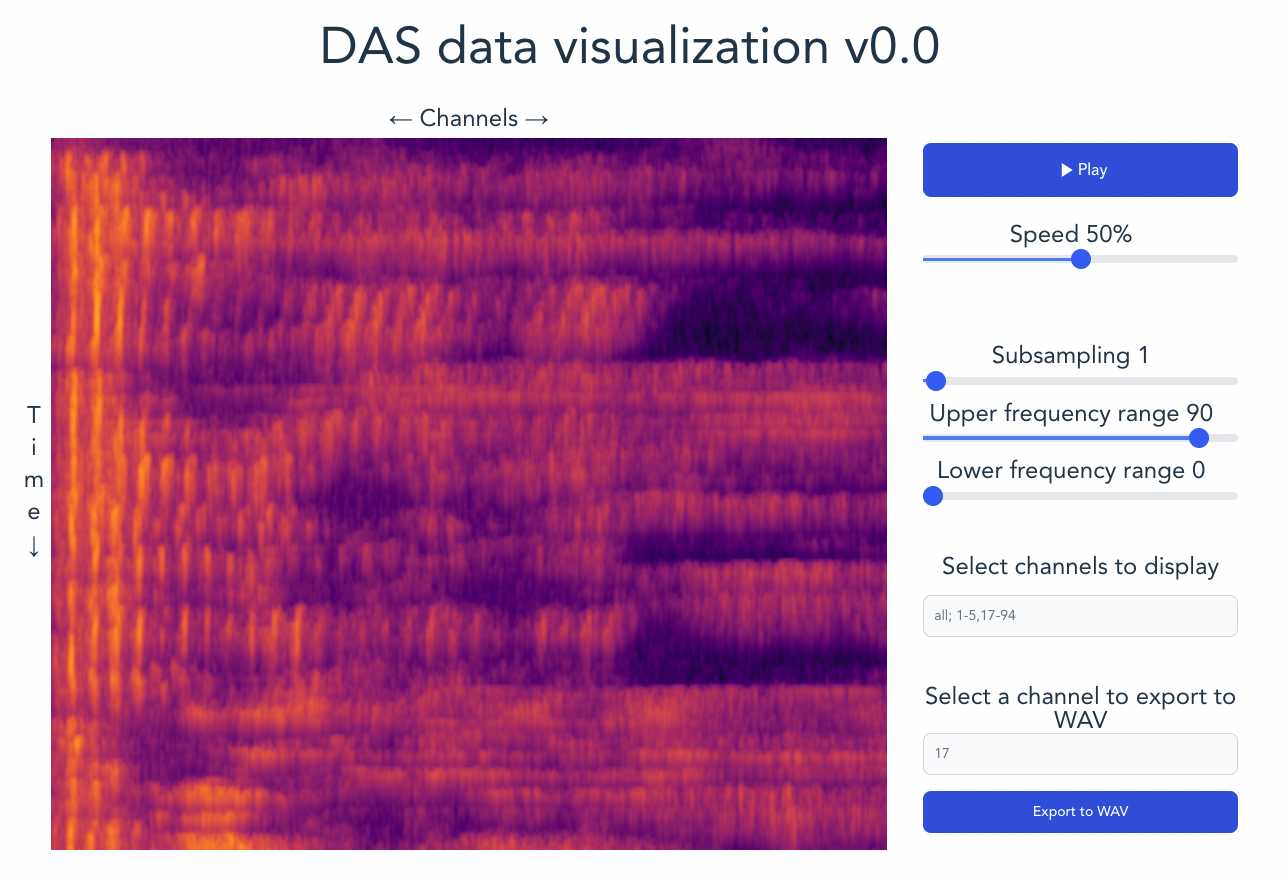
\includegraphics[width=0.8\linewidth]{obrazky/svelte_prototype.png}
        \caption{Prototype of DAS visualization application}
        \label{fig:prototypesvelte}
    \end{figure}
\end{frame}


\begin{frame}{Frame Title}
    \frametitle{Aplikácia }
    \begin{figure}
        \centering
        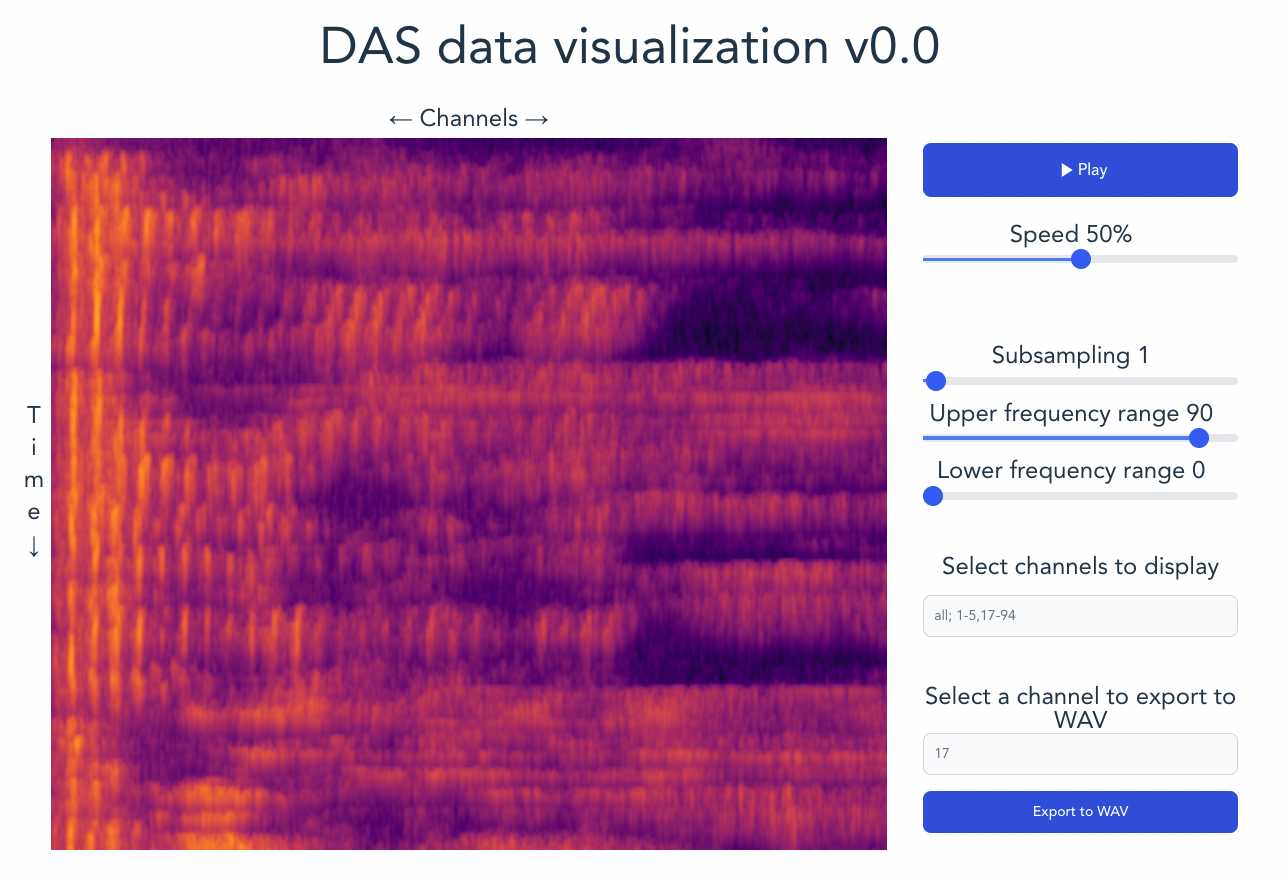
\includegraphics[width=0.8\linewidth]{obrazky/svelte_prototype.png}
        \caption{Prototype of DAS visualization application}
        \label{fig:prototypesvelte}
    \end{figure}
\end{frame}



% %%%%%%%%%%%%%
% \begin{frame} 
% 	\frametitle{Plošný spoj}
	
% 	\begin{columns}[T] 								% prostředí sloupce s umístěním nahoře
% 		\begin{column}{0.4\textwidth}		% první sloupec
% 			Obrázek znázorňuje model:\\[2ex]
% 			%
% 			\begin{itemize}
% 				\item Deska
% 				\item Součástky
% 				\item Signály
% 				\item Napájení
% 			\end{itemize}
% 		\end{column}
% 		%
% 		\begin{column}{0.6\textwidth}		% druhý sloupec
% 			\begin{figure}%	
% 				\centering
% 				\vspace{1cm}	              % horizontální mezera
% 				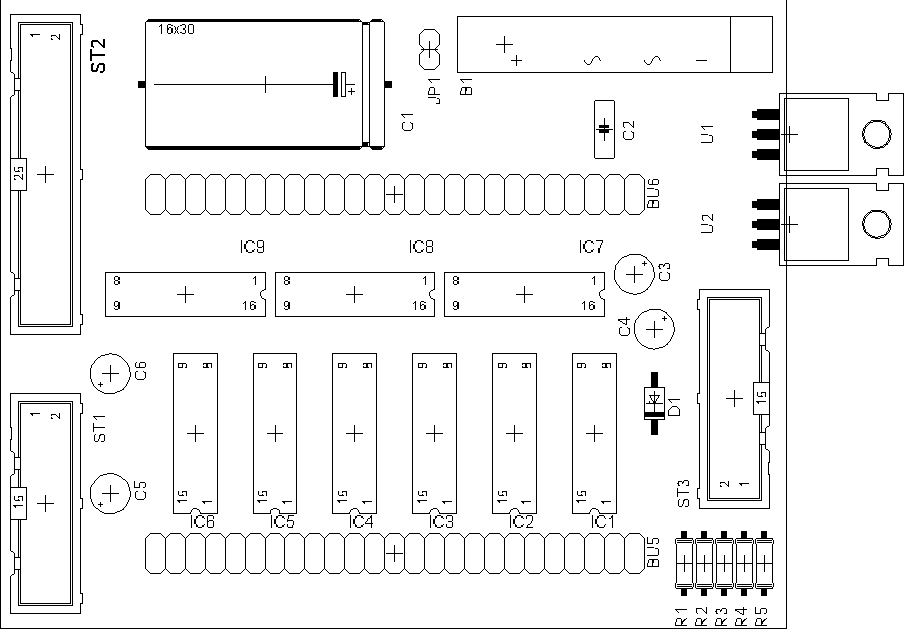
\includegraphics[width=0.8\columnwidth]{obrazky/soucastky}
% 				%lze vložit popisek, ale povetšinou je to v prezentaci zbytečné
% 				%\caption{Popisek obrázku}%
% 				%\label{obr:ukazka}
% 			\end{figure}
% 		\end{column}
% 	\end{columns}											% ukončení prostředí sloupce
% \end{frame}


%%%%%%%%%%%%%
% \begin{frame} 
% 	\frametitle{Výsledky}
% 	\vspace{1cm}
% 	\begin{table}[]
% 		\centering
% 		\caption{Výsledky měření mobilních sítí}
% 		\label{tab:tabulka}
% 			\begin{tabular}{lcc}
% 				\toprule
% 					Technologie  & Rychlost stahování [kB/s] & Rychlost nahrávání [kB/s] \\
% 				\midrule
% 					GPRS (2,5G)	& 7,2 	& 3,6\\
% 					UMTS 3G     & 48 		& 48\\
% 					HSPA (3,5G)	&	1\,706	&	720\\
% 					LTE (4G) 		& 40\,750 & 10\,750\\
% 				\bottomrule                                       
% 			\end{tabular}
% 	\end{table}
% \end{frame}


%%%%%%%%%%%%%
% \begin{frame} 
% 	\frametitle{Závěr}
% 	\dots
% \end{frame}


% podekovani
\begin{frame}[c] 
% bez nadpisu snímku
	\frametitle{\mbox{ }}
	\begin{center}
		{\Huge Ďakujem za pozornosť!}
	\end{center}
\end{frame}

% otázky oponenta
% \frame{
% \frametitle{Otázky oponenta}
% 	\emph{Jaká je souvislost Vašeho vzorce (1.2) s~Maxwellovými rovnicemi v~integrálním tvaru?}\\[2ex]
% 	%
% 	Již staří Římané\,\dots
% }

\end{document}
